% Условная компиляция для самостоятельной работы
\ifdefined\mainfile
    % Если это часть основного файла, не добавляем начало и конец документа
\else
    \documentclass[12pt, a4paper]{report}
    \usepackage{/Users/vladbelousov/Desktop/Semestr_4-FP-NSU/Настройка/library}
    \usepackage[utf8]{inputenc} % Подключение поддержки UTF-8
    \begin{document}
\fi

%%-------------------------------%%

\textbf{Опыт Поля продолжение}

Апертура интерференции: 

\begin{center}
    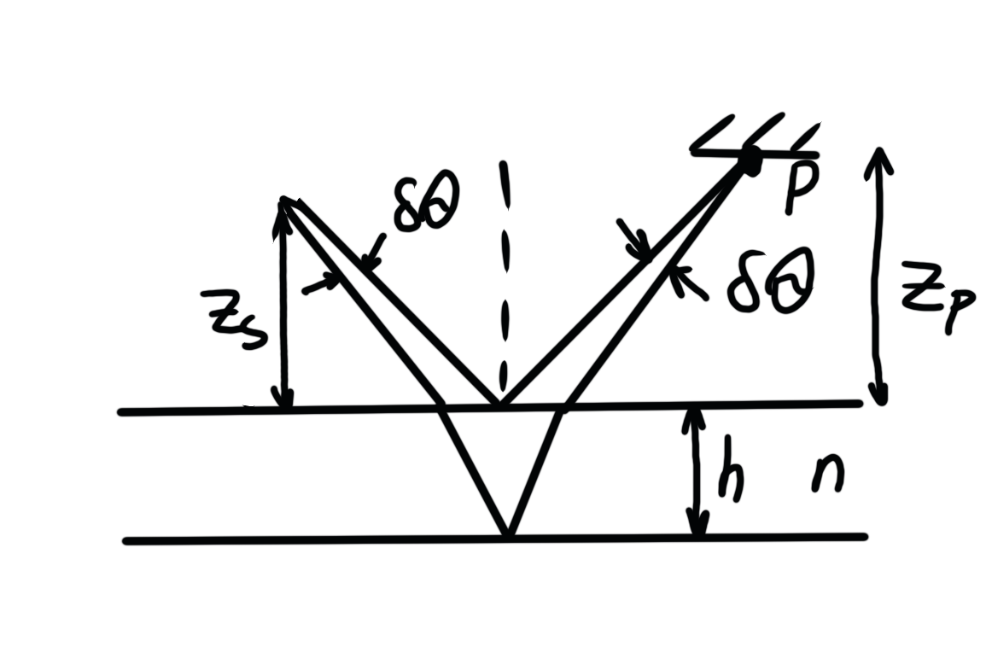
\includegraphics[width=0.5\textwidth]{/Users/vladbelousov/Desktop/Semestr_4-FP-NSU/ЭиО/Лекции_по_дням/image/163.png}
\end{center}

\[ 2 \omega = \delta \theta = \frac{2n}{z_s + z_p } \frac{ \cos  ^2 \theta_0 \sin  \theta_0 }{\sqrt{n ^2 - \sin  ^2 \theta_0}}   \] 

Проверим выполнение критерия видности интерференционной картины. \( V = \displaystyle  \frac{1}{2 }   \)  при \( \theta_{s _\perp }   \)  \( 2 \omega< \displaystyle  \frac{\lambda}{2 }   \) для этого сдвинем источник \( s ' \) на \( a_s  \) и добьемся разности хода лучей от \( s (\Delta r_s ) \)  и \( s ' (\Delta r _{s '} ) \), равной \( \displaystyle  \frac{\lambda}{2 }  \). Так как \( \delta \theta \ll 1 \text{ }  \left(  \displaystyle  \delta \theta \sim  \frac{\lambda}{z_s + z_p}  \right) \), то 

\begin{center}
    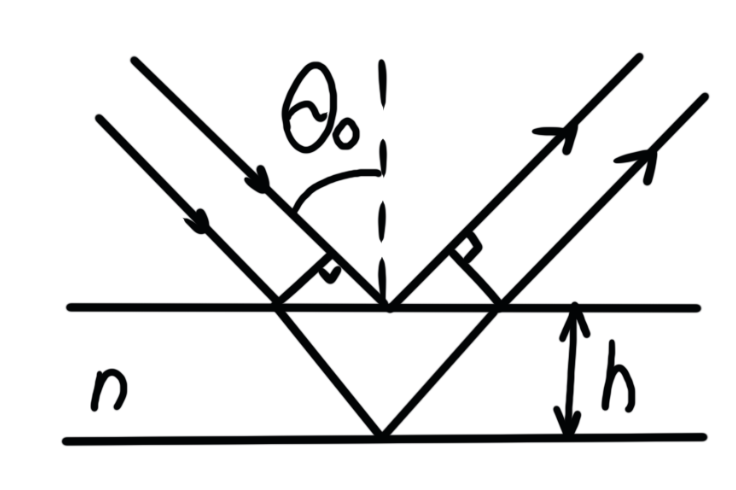
\includegraphics[width=0.4\textwidth]{/Users/vladbelousov/Desktop/Semestr_4-FP-NSU/ЭиО/Лекции_по_дням/image/164.png}
\end{center}

\[ \Delta r_s = \frac{2 h n }{\cos  \theta ' } - 2h \mathrm{tg } \theta ' \sin  \theta_0 + \frac{\lambda}{2 }    \] 

\begin{center}
    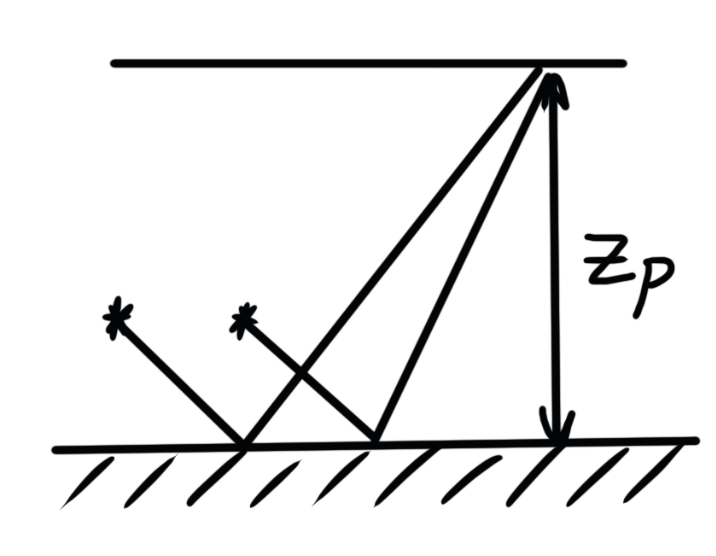
\includegraphics[width=0.4\textwidth]{/Users/vladbelousov/Desktop/Semestr_4-FP-NSU/ЭиО/Лекции_по_дням/image/165.png}
\end{center}

\[ a_s + (z_s + z_p ) \mathrm{ tg }  \theta_0 = (z_s + z_p ) \mathrm{tg }  (\theta_0 + \Delta \theta )   \] 
\[ a_s = (z_s + z_p ) ( \mathrm{ tg }  ( \theta_0 + \Delta \theta  ) - \mathrm{ tg }  \theta_0  ) \approx (z_s + z_p ) \frac{\Delta \theta }{\cos  ^2 \theta}  \] 

\[ \Delta r_{s ' }  - \Delta r_s = - \frac{\lambda}{2 }  \text{ }  \left( \text{это условие } V \approx \frac{1}{2}  \right) \] 

\[ 2h \sqrt{n ^2 - \sin  ^2 (\theta_0 + \Delta \theta  )} - 2h \sqrt{n ^2 - \sin  ^2 \theta_0 } \approx \frac{d}{d \theta_0 } (2h \sqrt{... })  \Delta \theta = 2h \frac{1}{2 }  \frac{ - 2 \sin  \theta_0 \cos  \theta_0 }{\sqrt{n ^2 - \sin  ^2 \theta_0 }} \Delta \theta_{ \max  } = - \frac{\lambda}{2} \Rightarrow    \] 
\[ \Rightarrow \Delta \theta_{ \max  } = \frac{ \lambda \sqrt{ n ^2 - \sin  ^2 \theta_0 }}{ 2 \cdot 2 h \sin  \theta_0 \cos  \theta_0}    \] 

\[ a_{s _{\max  } } = \frac{ z_s + z_p }{\cos  ^2 \theta_0 } \frac{ \lambda_0 \sqrt{ n ^2 - \sin ^2 \theta_0 } }{2 \cdot 2 h \sin  \theta_0 \cos  \theta_0 } ; \quad  \theta_{s _{\max  \perp } } = a_{s _{ \max  } } \cos  \theta_0       \] 

\[ a_{s _{ \max  \perp } }  - \delta \theta = \frac{ z_s + z_p }{ \cos  \theta_0 } \frac{\lambda_0}{2 }  \frac{\sqrt{ n ^2 - \sin  ^2 \theta_0 } }{2 h \sin  \theta_0 \cos  \theta_0 } \frac{ 2 h }{z_s + z_p } \frac{ \cos  ^2 \theta_0 \sin  \theta_0 }{\sqrt{n ^2 - \sin  ^2 \theta_0 } }= \frac{\lambda_0}{2}       \] 

Видность интерференционной картины в схеме (смотреть две лекции назад) (в центре картины): 

\[ V = \left\lvert \mathrm{ sinc } \frac{k d a_s }{ 2 L_s }    \right\rvert \text{ Если } V \approx \frac{1}{2  } \Rightarrow    \] 
\[ \Rightarrow \frac{ 2 \pi d a_s }{\lambda_0 2 L_s } = \frac{\pi}{2 }  \Rightarrow d = \frac{\lambda}{\displaystyle  2 \frac{a_s}{L_s} }   \] 

Интерференционные полосы, локализованные на поверхности пленки:

\begin{center}
    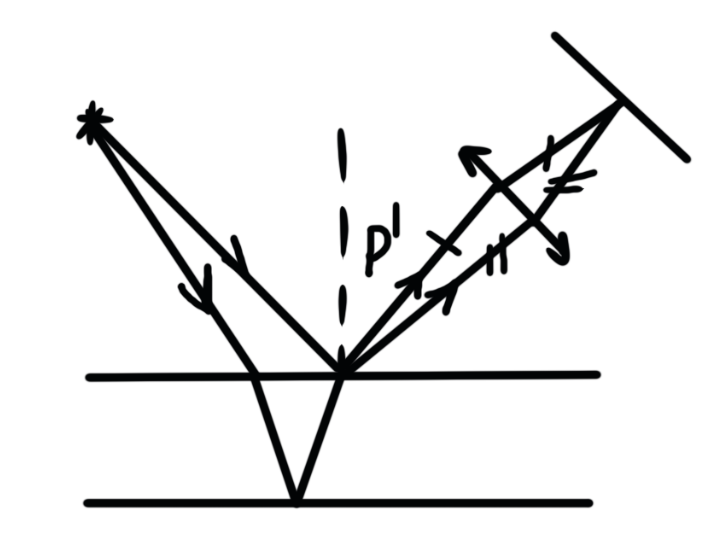
\includegraphics[width=0.4\textwidth]{/Users/vladbelousov/Desktop/Semestr_4-FP-NSU/ЭиО/Лекции_по_дням/image/166.png}
\end{center}
\( p \) и \( p' \) - сопряженные точки \( \Rightarrow  \Delta r \) лучей, идущих из \( p ' \) в \(  p \)  - одинакова.

\begin{center}
    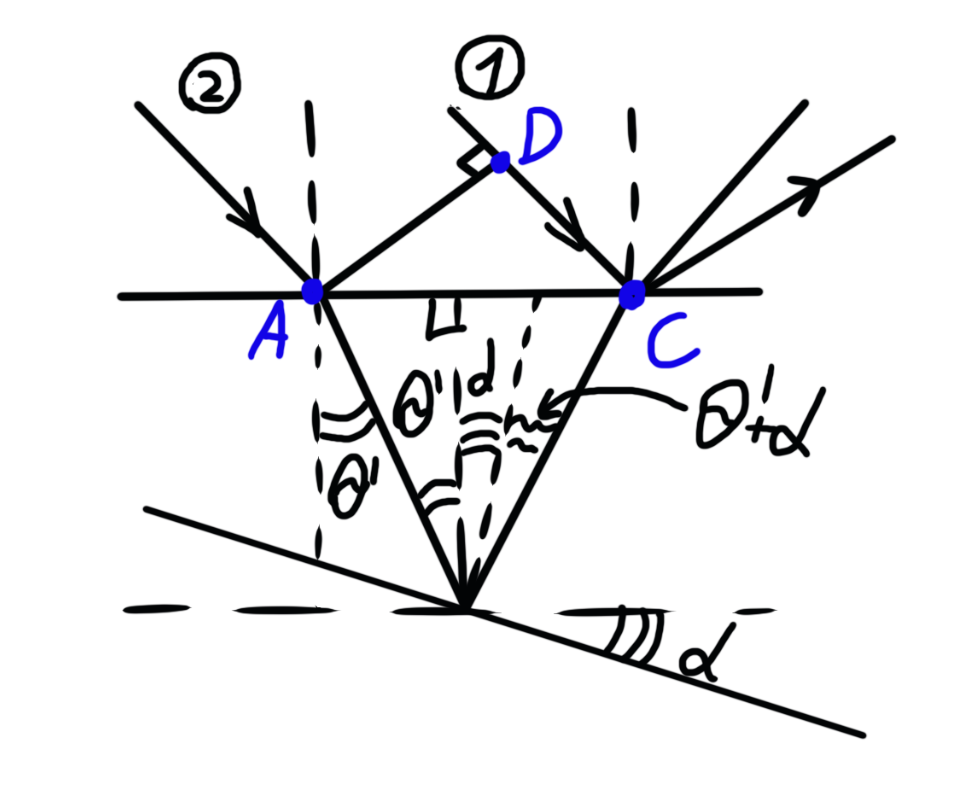
\includegraphics[width=0.5\textwidth]{/Users/vladbelousov/Desktop/Semestr_4-FP-NSU/ЭиО/Лекции_по_дням/image/167.png}
\end{center}
\[ \Delta r = n (\left\lvert  AB  \right\rvert + \left\lvert BC \right\rvert) - \left\lvert   CD\right\rvert  = h \left( \frac{h (x )}{ \cos  \theta '} + \frac{ h (x )}{\cos (\theta ' + 2 \alpha ) }    \right) - (h (x ) \mathrm{ tg }  \theta ' + h(x ) \mathrm{tg }  ( \theta ' + 2 \alpha )  ) \sin \theta_0 + \frac{\lambda}{2 } = \] 
\[ = \left[ \sin  \theta_0 = n \sin \theta ' (\text{закон Снелиуса} ) \right] = n h (x ) \left(  \cos  \theta ' + \frac{1}{ \cos  (\theta ' + 2 \alpha )} - \frac{ \sin (\theta '  + 2 \alpha ) \sin  \theta ' }{ \cos  (\theta ' + 2\alpha)}   \right) + \frac{\lambda_0}{2} = \] 
\[ =n h(x ) \frac{ \cos  \theta ' \cos  ( \theta ' + 2 \alpha ) - \sin  ( \theta ' + 2 \alpha ) \sin  \theta ' + 1 }{ \cos ( \theta ' + 2\alpha)}  + \frac{\lambda_0}{2 } =  n h(x ) \frac{ \cos  (2 \theta ' + 2 \alpha ) + 1 } {\cos  ( \theta ' + 2\alpha )}     + \frac{\lambda_0}{2 }   =  \]  
\[ = \left[ \text{разложение по } \alpha \ll 1 \right] = n h(x ) \bigg\{ 2 \cos  \theta ' + \underbrace{\frac{ \cos ( 2 \theta ' + 2 \alpha )+1}{\cos  (\theta ' + 2 \alpha )} - 2 \cos  \theta'}_{\text{поправка} } \bigg\} + \frac{\lambda_0}{2}  \] 

\[ \delta = \cos  2 \theta ' \left(  1 - \frac{( 2 \alpha ) ^2 }{2 }  \right) - \sin  \theta ' \cdot 2 \alpha + 1 - 2 \cos  \theta '  \] 

\[ \left( \cos  \theta ' \left(  1 - \frac{ ( 2 \alpha ) ^2 }{2 }  \right) - \sin  \theta ' \cdot 2 \alpha  \right) =  \] 
\[\kern-1cm =\frac{(2 \cos  ^2 \theta ' -1 )(1 - 2 \alpha ^2 )- 2 \sin  \theta ' \cos  \theta' \cdot 2 \alpha - 2 \cos  ^2 \theta ' ( 1 - 2 \alpha ^2 )+ 2 \cos  \theta ' \sin  \theta ' \cdot 2\alpha + 1 }{\cos  ( \theta ' 2\alpha )}  = \frac{ 2 \alpha ^2 }{ \cos  ( \theta ' + 2\alpha )}  \] 

\[ \Delta r (x ) = n h(x ) \left[  2 \cos  \theta ' + \frac{ 2 \alpha ^2 }{ \cos  \rho ' }  \right] + \frac{\lambda_0}{2}  \] 

Чтобы наличие \( \alpha  \) не усложняла интерференционную картину, \( \theta '  \) выберем близким к 0 \( \Delta r (x ) \approx \displaystyle  2 n h(x ) + \frac{\lambda_0}{2}  \) 

\begin{definition}
    Г.М.Т., в которых  \( \Delta r (x ) = 2 n h (x ) + \displaystyle  \frac{\lambda}{2 }  = m \lambda_0 \), образуют линии равной толщ
\end{definition}

\section{ Дифракция света}

\begin{center}
    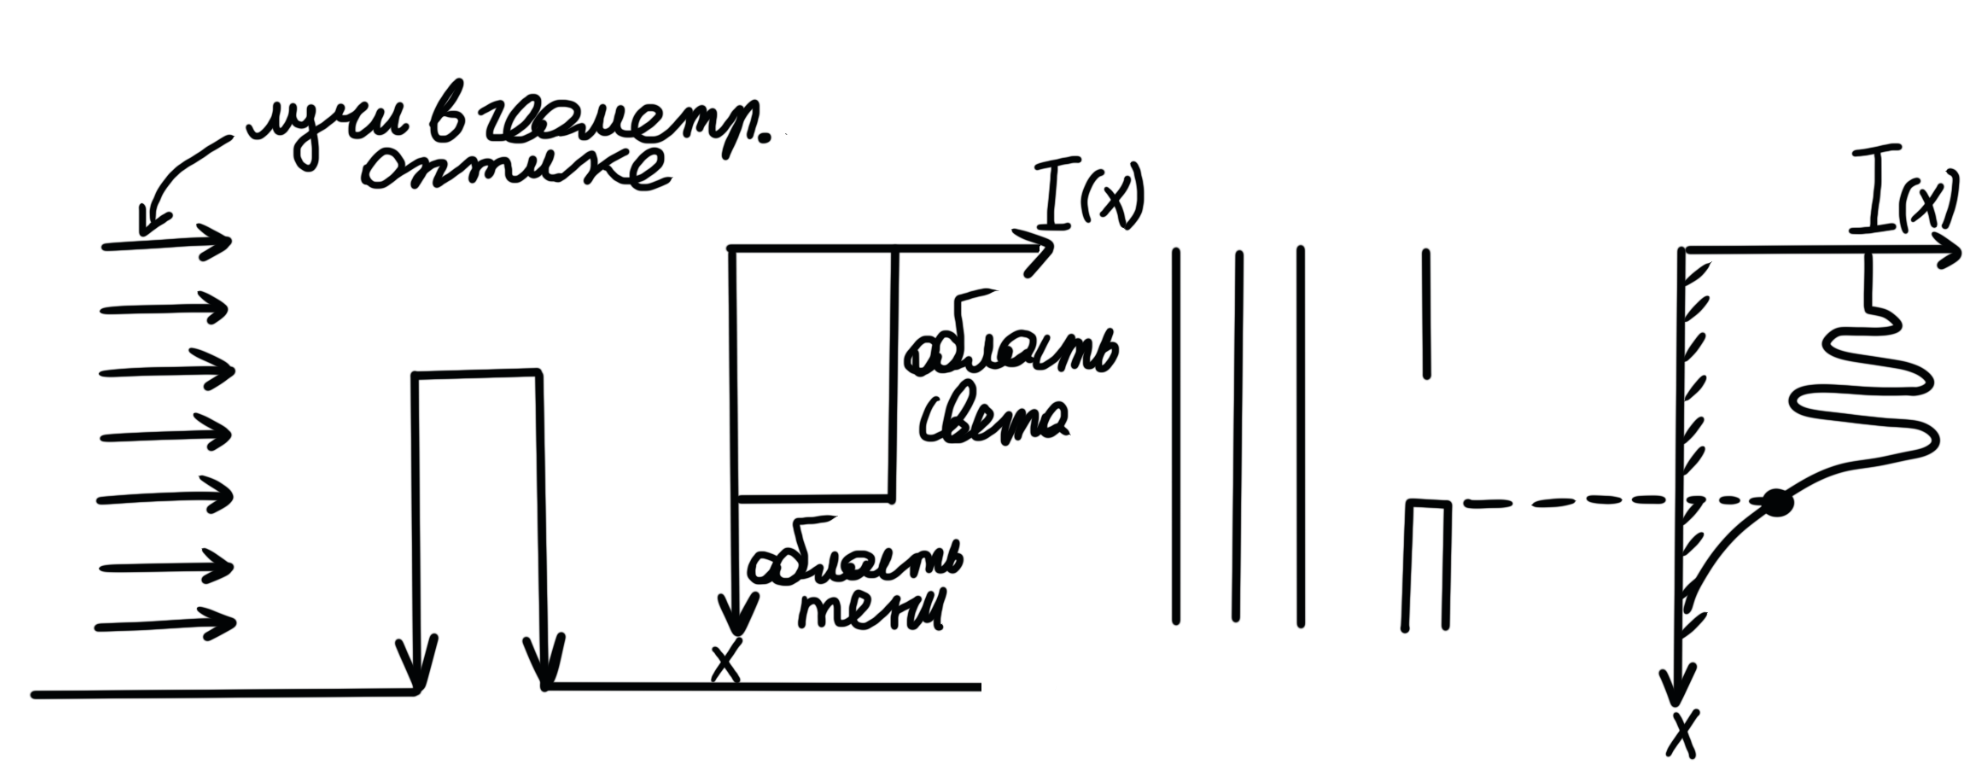
\includegraphics[width=0.8\textwidth]{/Users/vladbelousov/Desktop/Semestr_4-FP-NSU/ЭиО/Лекции_по_дням/image/168.png}
\end{center}

Принцип Гюйгенса - каждая точка волнового фронта является источников вторичных волн, а сложение вторичных волн формирует диффракционную картину. Формулировка  Френеля принципа Гюйгенса: 

\begin{center}
    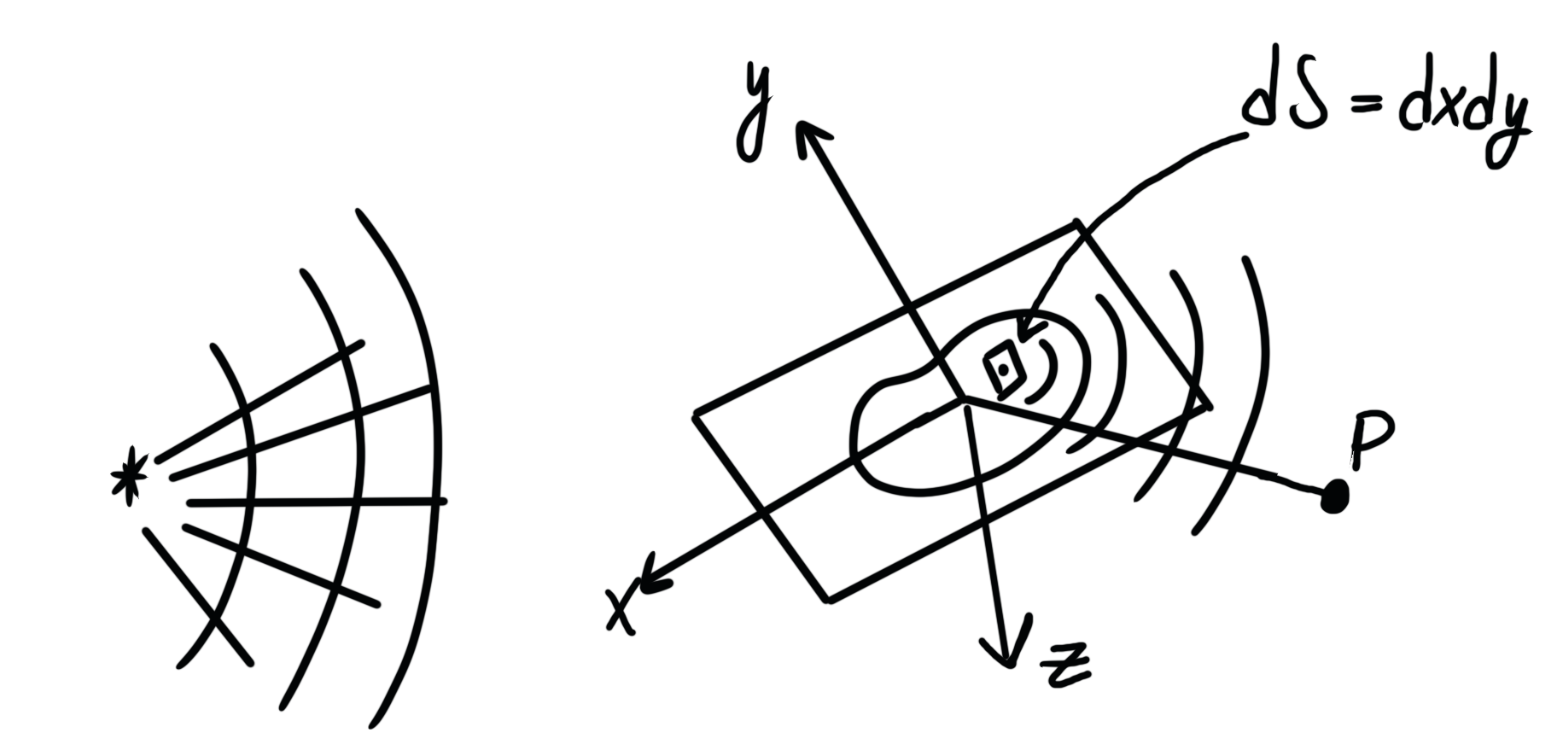
\includegraphics[width=0.6\textwidth]{/Users/vladbelousov/Desktop/Semestr_4-FP-NSU/ЭиО/Лекции_по_дням/image/169.png}
\end{center}

\[ \int  d E_p ( \text{от } dS       ) = \int E \kern-1cm\underbrace{(s )}_{(x,y,z )\text{ в отверстии} }  \kern-1cm\frac{e ^{ ik R - i \omega t } }{R } \mathbb{K}     (\alpha ) d S _n   \] 
, где \( d S_n\)  - проекция \( d S \) на направления перпендикулярное лучам.

\begin{center}
    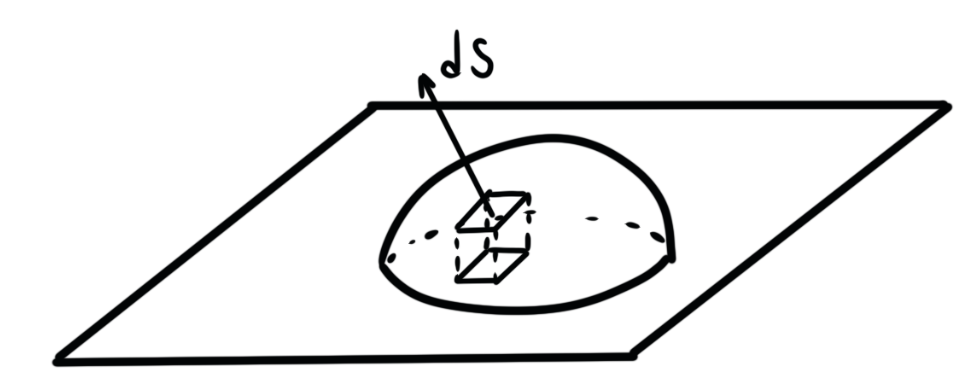
\includegraphics[width=0.5\textwidth]{/Users/vladbelousov/Desktop/Semestr_4-FP-NSU/ЭиО/Лекции_по_дням/image/170.png}
\end{center}


%%-------------------------------%%

% Закрытие документа, если файл компилируется отдельно
\ifdefined\mainfile
    % Если это основной файл, не нужно заканчивать документ
\else
    \end{document}
\fi